\documentclass{article}
\usepackage{amsmath,amssymb}   % 数学公式
\usepackage{graphicx}          % 插入图片
\usepackage{hyperref}          % 超链接
\usepackage{geometry}          % 页边距设置
\usepackage{float}             % 控制图形位置
\usepackage{caption}           % 自定义标题
\geometry{a4paper, margin=1in}

\title{Reinforcement Learning Homework3\\[0.5em]
\large Project 1: Grid World Wind Simulation Task\\
\large Project 2: Brick Breaking Game Task}
\author{Pang Liu}
\date{March 30, 2025}

\begin{document}

\maketitle

\section{Introduction}
This report documents the development and analysis of two distinct projects implemented in Python. The first project focuses on a grid world environment with stochastic wind dynamics, where multiple reinforcement learning algorithms (SARSA, Q-learning, and Monte Carlo) are employed to learn an optimal policy for reaching a designated goal. The second project is a discrete version of the classic Breakout (brick breaking) game, where a Q-learning agent is trained to control a paddle and clear bricks. The experiment details the problem setups, state-action spaces, reward settings, iterative update rules, implementation details, and experimental results for both tasks.

\section{Grid World Wind Simulation Task}
\subsection{Problem Description and Environment Setup}
In this task, a grid world environment with dimensions $10 \times 10$ is constructed. The environment is adapted from \textit{Exercise 6.9} (Windy Gridworld with King’s Moves) and \textit{Exercise 6.10} (Stochastic Windy Gridworld) in \emph{Reinforcement Learning: An Introduction} (Sutton \& Barto). Specifically, the experiment combines:
\begin{itemize}
    \item \textbf{King’s Moves (Exercise 6.9):} The agent can move in 8 possible directions plus a ``stay'' action, allowing for diagonal movements.
    \item \textbf{Stochastic Wind (Exercise 6.10):} Each column has a base wind strength, which can increase by 1, remain unchanged, or decrease by 1 with equal probability.
\end{itemize}

The agent starts at position $(5,3)$ and must reach the goal at $(5,8)$ while contending with wind pushing it upward.

\subsection{State and Action Space}
\subsubsection{State Space}
The state is represented by the agent’s position on the grid:
\[
S = (r, c) \quad \text{with } r \in \{0,1,\dots,9\}, \; c \in \{0,1,\dots,9\}.
\]

\subsubsection{Action Space}
Due to the King’s Moves, the action set consists of 9 possible moves:
\[
\text{Actions} = \{(0,0),\, (-1,0),\, (-1,1),\, (0,1),\, (1,1),\, (1,0),\, (1,-1),\, (0,-1),\, (-1,-1)\},
\]
where each tuple represents the change in row and column. After applying the action, the stochastic wind further adjusts the row value by pushing the agent upward.

\subsection{Reward Setting}
The reward is defined as:
\[
r_t =
\begin{cases}
-1, & \text{if the agent moves without reaching the goal},\\[1mm]
0, & \text{if the agent reaches the goal.}
\end{cases}
\]
Thus, the agent is penalized by $-1$ per step, which encourages the experiment to reach the goal in as few steps as possible.

\subsection{Reinforcement Learning Algorithms and Iterative Updates}
The implementation in \texttt{1\_primary.py} uses three reinforcement learning methods:
\begin{itemize}
    \item \textbf{SARSA:} The Q-value update is
    \[
    Q(s,a) \leftarrow Q(s,a) + \alpha \Bigl[r + \gamma Q(s',a') - Q(s,a)\Bigr],
    \]
    where $(s,a)$ is the current state-action pair and $(s',a')$ is the next state and action.
    \item \textbf{Q-learning:} The off-policy update rule is
    \[
    Q(s,a) \leftarrow Q(s,a) + \alpha \Bigl[r + \gamma \max_{a'} Q(s',a') - Q(s,a)\Bigr],
    \]
    which uses the maximum Q-value in the next state.
    \item \textbf{Monte Carlo:} The Q-values are updated based on the averaged returns from complete episodes.
\end{itemize}

\subsection{Experimental Testbed and Results}
The experiment was carried out over multiple episodes (e.g., 500 episodes per run) and several runs (e.g., 3 runs) to ensure robustness of the performance metrics. The testbed includes a well-defined grid world, a wind simulation based on column-specific base wind with stochastic variations, and an implementation of the three RL algorithms. Figure~\ref{fig:figure1} shows the learning curves (average reward and success rate vs. episodes) obtained from the experiment. Here, the orange curve represents Q-learning, the blue curve represents SARSA, and the green curve represents Monte Carlo.

\begin{figure}[H]
    \centering
    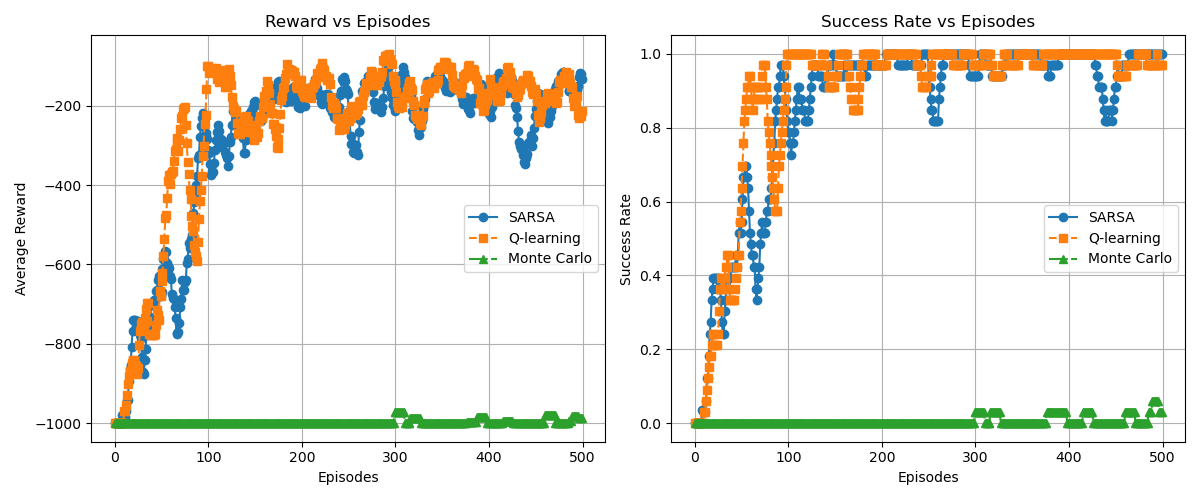
\includegraphics[width=0.8\textwidth]{Figure_1.png}
    \caption{Learning curves for the grid world wind simulation task (from \texttt{1\_primary.py}). Left: Average reward vs. episodes. Right: Success rate vs. episodes.}
    \label{fig:figure1}
\end{figure}

\noindent\textbf{Analysis of the Curves:}
\begin{itemize}
    \item \textbf{Q-learning (orange):} \\
          The average reward increases rapidly, indicating that the experiment quickly learns to minimize step penalties by reaching the goal in fewer steps. The success rate climbs sharply and remains close to 1.0, which suggests that once Q-learning finds an efficient path, the goal is consistently reached. The off-policy nature of Q-learning allows value estimates to be propagated more aggressively from the goal backwards, thereby accelerating convergence.
    \item \textbf{SARSA (blue):} \\
          Although the success rate converges to a high value, it does so more gradually compared to Q-learning. The average reward initially lags behind that of Q-learning because SARSA updates using the actual action taken (on-policy), which leads to more cautious exploration under stochastic wind conditions. Over time, SARSA's performance approaches that of Q-learning, demonstrating that near-optimal paths are eventually learned.
    \item \textbf{Monte Carlo (green):} \\
          The method remains at a very low success rate and yields highly negative average rewards over the limited number of episodes. This outcome is attributed to the need for complete episodes to update the action values; in a large or stochastic environment, successful episodes are rare early in the experiment. With a larger number of episodes or an alternative exploration strategy, the Monte Carlo method might eventually converge, but under the current settings it struggles.
\end{itemize}

\section{Brick Breaking Game Task}
\subsection{Problem Description and Environment Setup}
The second project implements a discrete version of the Breakout game as defined in \texttt{2\_secondary.py}. The testbed for the experiment includes:
\begin{itemize}
    \item A $10 \times 10$ grid.
    \item A paddle fixed at the bottom row that can move left or right.
    \item Bricks arranged in the top row, represented by a bit mask.
    \item A ball that moves with fixed velocity, bouncing off walls, bricks, and the paddle.
\end{itemize}

The experiment is conducted in a simulated environment where the paddle is controlled by a Q-learning agent, and game dynamics (ball movement, collision detection, and reward distribution) are implemented following the predefined rules. This experiment is related to the final project, which will address a more complicated breakout game with a larger state space. To evaluate Q-learning on a simpler testbed, the breakout game is abstracted to a much smaller state space. An important improvement in this testbed is the careful design of the state space to achieve efficient learning.

\subsection{Environment Visualization}
To help the reader understand the experimental testbed, Figures~\ref{fig:figure3} and \ref{fig:figure4} below show screenshots of the breakout game environment. Figure~\ref{fig:figure3} displays the game in progress, while Figure~\ref{fig:figure4} shows the game state after clearing all bricks.

\begin{figure}[H]
    \centering
    \begin{minipage}[t]{0.48\textwidth}
        \centering
        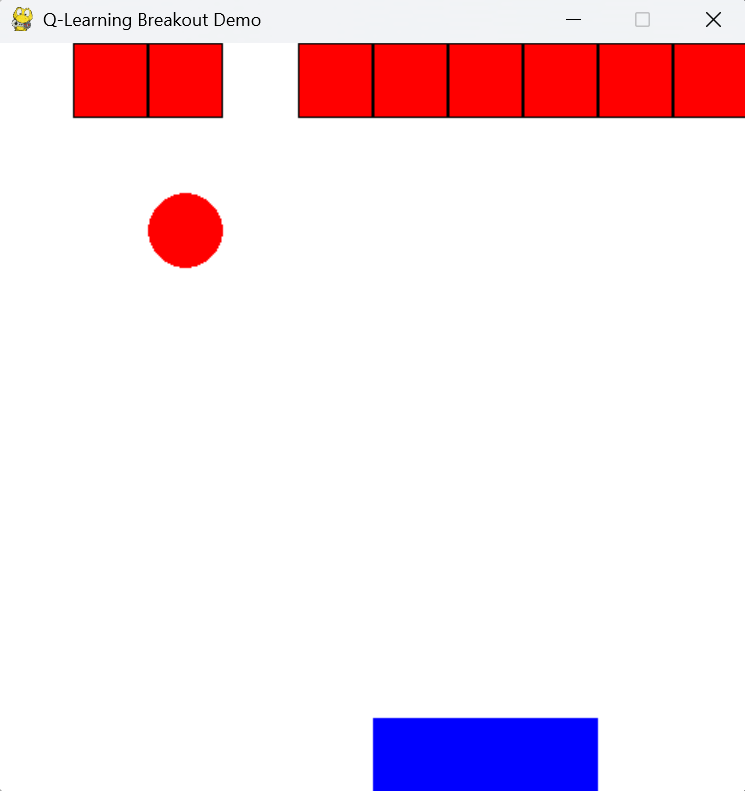
\includegraphics[width=\textwidth]{Figure_3.png}
        \caption{Breakout game in progress.}
        \label{fig:figure3}
    \end{minipage}
    \hfill
    \begin{minipage}[t]{0.48\textwidth}
        \centering
        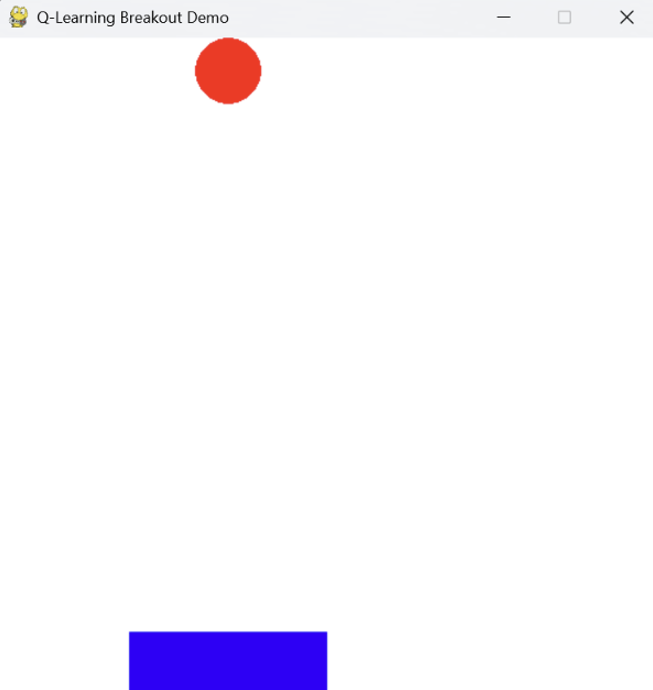
\includegraphics[width=\textwidth]{Figure_4.png}
        \caption{Breakout game after clearing all bricks.}
        \label{fig:figure4}
    \end{minipage}
\end{figure}

\subsection{State and Action Space}
\subsubsection{State Space}
The state is represented by a tuple that captures the key elements of the game:
\[
S = (\text{ball}_x, \text{ball}_y, v_x, v_y, \text{paddle}_x, \text{brick\_count}),
\]
where:
\begin{itemize}
    \item $\text{ball}_x, \text{ball}_y$: The position of the ball.
    \item $v_x, v_y$: The ball's velocity components.
    \item $\text{paddle}_x$: The leftmost position of the paddle.
    \item $\text{brick\_count}$: The number of bricks remaining in the top row.
\end{itemize}

\subsubsection{Action Space}
There are three possible actions for the paddle:
\begin{itemize}
    \item \textbf{0:} No movement.
    \item \textbf{1:} Move paddle left.
    \item \textbf{2:} Move paddle right.
\end{itemize}

\subsection{Reward Setting}
The reward design in the Breakout game is as follows:
\begin{itemize}
    \item A small step penalty of $-0.1$ per move.
    \item A reward of $+5$ when the ball hits a brick (and the brick is removed).
    \item A reward of $+1$ when the ball hits the paddle.
    \item A final reward of $+10$ if all bricks are cleared (victory) or a penalty of $-10$ if the ball is lost (failure).
\end{itemize}

\subsection{Q-learning Iterative Update}
The Q-learning algorithm is implemented with an $\epsilon$-greedy strategy (with $\epsilon$ decaying linearly) and uses the update rule:
\[
Q(s,a) \leftarrow Q(s,a) + \alpha \Bigl[r + \gamma \max_{a'} Q(s',a') - Q(s,a)\Bigr].
\]
Here,
\begin{itemize}
    \item $\alpha$ is the learning rate.
    \item $\gamma$ is the discount factor.
    \item $r$ is the reward received after taking action $a$ in state $s$.
    \item $s'$ is the next state, and $\max_{a'} Q(s',a')$ represents the maximum Q-value for the next state.
\end{itemize}

\subsection{Experimental Testbed and Results}
The experiment was conducted over a large number of episodes (e.g., 100,000 episodes) with the Q-learning agent, and performance metrics (episode reward and success rate) were recorded. Figure~\ref{fig:figure2} displays the learning curves for the Breakout game, showing the evolution of episode rewards and success rate (defined as clearing all bricks) with a moving average applied for smoother visualization.

\begin{figure}[H]
    \centering
    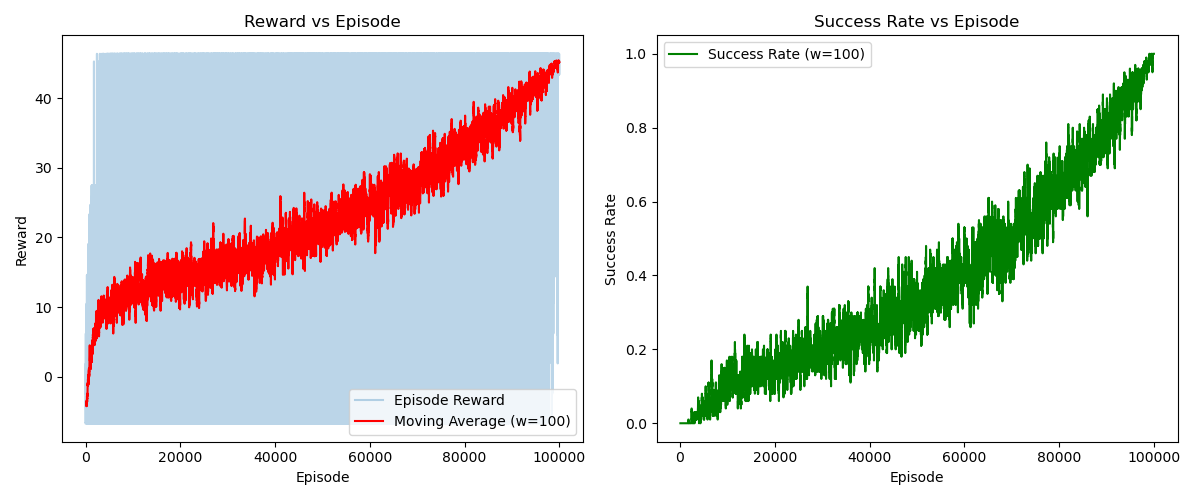
\includegraphics[width=0.8\textwidth]{Figure_2.png}
    \caption{Learning curves for the Breakout game task (from \texttt{2\_secondary.py}).}
    \label{fig:figure2}
\end{figure}

The experimental results indicate that the Q-learning agent effectively learns to control the paddle. The learning curves reflect an increase in average reward and success rate over episodes, while the game demonstration confirms that the agent can clear all bricks.

\subsection{Future Extensions toward a Full Breakout Game}
In future work, the insights gained from this simplified Breakout environment will be used to design a more complete version of the game with a larger state space and additional features (e.g., multiple rows of bricks, advanced collision physics, power-ups). The next step is to extend Q-learning to more powerful function approximators such as Deep Q-Networks (DQN), which can handle high-dimensional inputs effectively. This approach will allow the policy to generalize better in complex environments, paving the way for a robust solution to the full Breakout game.

\section{Conclusion}
This report presents two reinforcement learning applications developed as part of Homework3. The grid world wind simulation task incorporates a stochastic wind environment and King’s Moves, combining ideas from Exercises 6.9 and 6.10 in \emph{Reinforcement Learning: An Introduction}. The experiment employs SARSA, Q-learning, and Monte Carlo methods to guide the agent toward a target, with detailed descriptions of state-action space, reward design, and iterative update rules. The learning curves reveal that Q-learning demonstrates the fastest convergence, SARSA converges more cautiously, and Monte Carlo struggles under the given episode limit.

The Breakout game task uses a Q-learning agent to control a paddle in a discrete grid environment, with clearly defined state space, action space, reward settings, and update formulas. The experimental results and visualizations confirm that the agent can successfully learn to clear all bricks. In addition, the simplified environment design offers valuable insights for scaling to a full Breakout game and transitioning from tabular Q-learning to deep reinforcement learning methods such as DQN.

\section{References}
\begin{itemize}
    \item Sutton, R. S., \& Barto, A. G. (2018). \emph{Reinforcement Learning: An Introduction} (2nd Edition).
    \item Additional online resources and documentation for Python, NumPy, Matplotlib, and Pygame.
\end{itemize}

\end{document}
